\documentclass[11pt]{article}

\usepackage{a4wide}
\usepackage{mathptm}
\usepackage{xspace}
\usepackage{amsmath}
\usepackage{graphicx}
\usepackage{algorithm}
\usepackage{algpseudocode}
\usepackage{tikz}
\usepackage{tkz-graph}
\usetikzlibrary{shapes.misc, positioning}
\usepackage{listings}
\usepackage{color}

\definecolor{dkgreen}{rgb}{0,0.6,0}
\definecolor{gray}{rgb}{0.5,0.5,0.5}
\definecolor{mauve}{rgb}{0.58,0,0.82}

\lstset{frame=tb,
  language=Java,
  aboveskip=3mm,
  belowskip=3mm,
  showstringspaces=false,
  columns=flexible,
  basicstyle={\small\ttfamily},
  numbers=left,
  numberstyle=\tiny\color{gray},
  keywordstyle=\color{blue},
  commentstyle=\color{dkgreen},
  stringstyle=\color{mauve},
  breaklines=true,
  breakatwhitespace=true,
  tabsize=3
}
\begin{document}

\title{DAT110 Oblig 4 Part A-C}

\author{Joakim Johesan and Eirik Alvestad}

\maketitle

\begin{abstract}
An Arduino access controll system with cloud based features, enabled by the use of a cloud server with a REST API. Designed and written with TinkerCad, Java, C++ and using Gson and the Spark framework.
\end{abstract}

\input{./sections/introduction}

\section{Access Control Design Model}
\label{sec:background}

(~1 page) presenting your finite state machine for the access control device that you developed in Part A. This section should contain a figure showing the finite state machine, and contain a short description of it and the main design choices you have made.



\section{Access Control Hardware/Software Implementation }
(~1.5 pages) explaining how you have implemented the hardware and the software of the access control device. The section should contain a figure presenting your TinkerCAD circuit design


\begin{figure}[H]
  \centering
  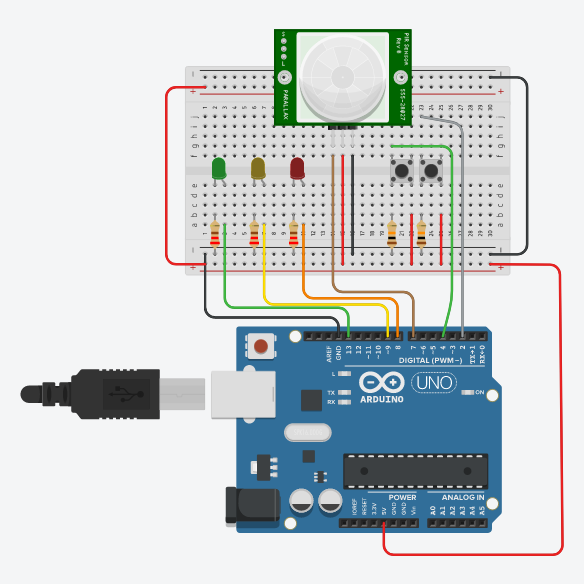
\includegraphics[scale=0.5]{figs/ArduinoSnapshot.png}
  \caption{Arduino koblingdiagram}
  \label{fig:Arduino}
\end{figure}

\pagebreak

\section{REST API cloud service}
We implemented the cloud service using the spark/java framework, which makes it easy to implement a REST api.
We used the framework so that the cloud service makes it possible for the access control device to register attempts to access the system in an access log, and to be able to change the access code and retrieve the current access code.
The task was well written and we set up the routes the way the task specified. \\

The routes was set up using the spark framework which allows us to specify the operation type (get, post, put, etc..) and the url in a easy way.
The access attempts is collected in memory, which means that the information is only stored for as long as the program is running. Each log message received via the POST HTTP operation is given a unique identifier. We used a Concurrent HashMap for storing the log-messages received from the device and an Atomic Integer for keeping track of the identifier like the task suggested. The hash-map uses the identifier as the key for the log-message.
Like the task specified we used the Gson-library. We used two of the methods of this library(toJson, fromJson).
toJson: converts a java object into a Json representation
fromJson: converts a Json representation into a java object that the code specified.


\section{Device Communication}
We implemented the network communication in the access control device by using some of the services implemented in the cloud service.\\

The first task was to implement a way for the device to obtain the current access code. We did this by establishing a connection to the cloud-service and issue the appropriate HTTP GET request.
\\
For this we used java socket to establish a connection to the cloud-service. We then constructed the get request consisting of the URL that matches the cloud-service route that returns the current access code, and write it to the ouput stream. We then take the response and iterate through it to get the body of the response, create a AccessCode object using the Gson-library and return that object.\\

The second task was to implement a way for the device to  issue a HTTP POST request on the service in order to add a log access entry for the message.
For this we used java socket again to establish a connection to the cloud-service. When using the cloud service it required us to create a post request where the body consists of a json represented object, we did this by first creting a java AccessMessage object from the parameter message, and convert it to a json representation using the Gson-library. We then constructed the post request consisting of the URL that matches the cloud-service route that allows us to save a message to the hashmap. We  put the json representation of the message in the body of the request and wrote to the outputstream.
   


\section{System Testing}
While we implemented the operations the task required us to implement, it was important for us to be able to test what we just implemented to make sure it was correct. We did this mostly using the postman tool that the task suggested. The postman tool allowed us to easily paste in a the desired url and choose if we wanted to post/get/put to the specified url. The postman tool was the most useful when testing the post method because it allows us to insert a json representation of a object directly in the body of the request.\\
When we were done implementing the cloud service and started implementing the device network communication the testing consisted more of running the device and manually testing the different functions it should be able to perform. But here we also used the postman tool to test the doGetAccessCode() method, because the testing required us to change the access code, and this as easily done using the postman tool.

\section{Conclusions }
(~1/4 page) briefly summing of the status of the project, including things that was not completed or which the group did not manage to get to work properly.

\bibliographystyle{plain}

\end{document}